% Graphic for TeX using PGF
% Title: /home/yy12135/Google Drive/Writings/First-year-review_20150422/Pics/LeakyCoffee.dia
% Creator: Dia v0.97.2
% CreationDate: Tue Mar  3 14:05:39 2015
% For: yy12135
% \usepackage{tikz}
% The following commands are not supported in PSTricks at present
% We define them conditionally, so when they are implemented,
% this pgf file will use them.
\ifx\du\undefined
  \newlength{\du}
\fi
\setlength{\du}{15\unitlength}
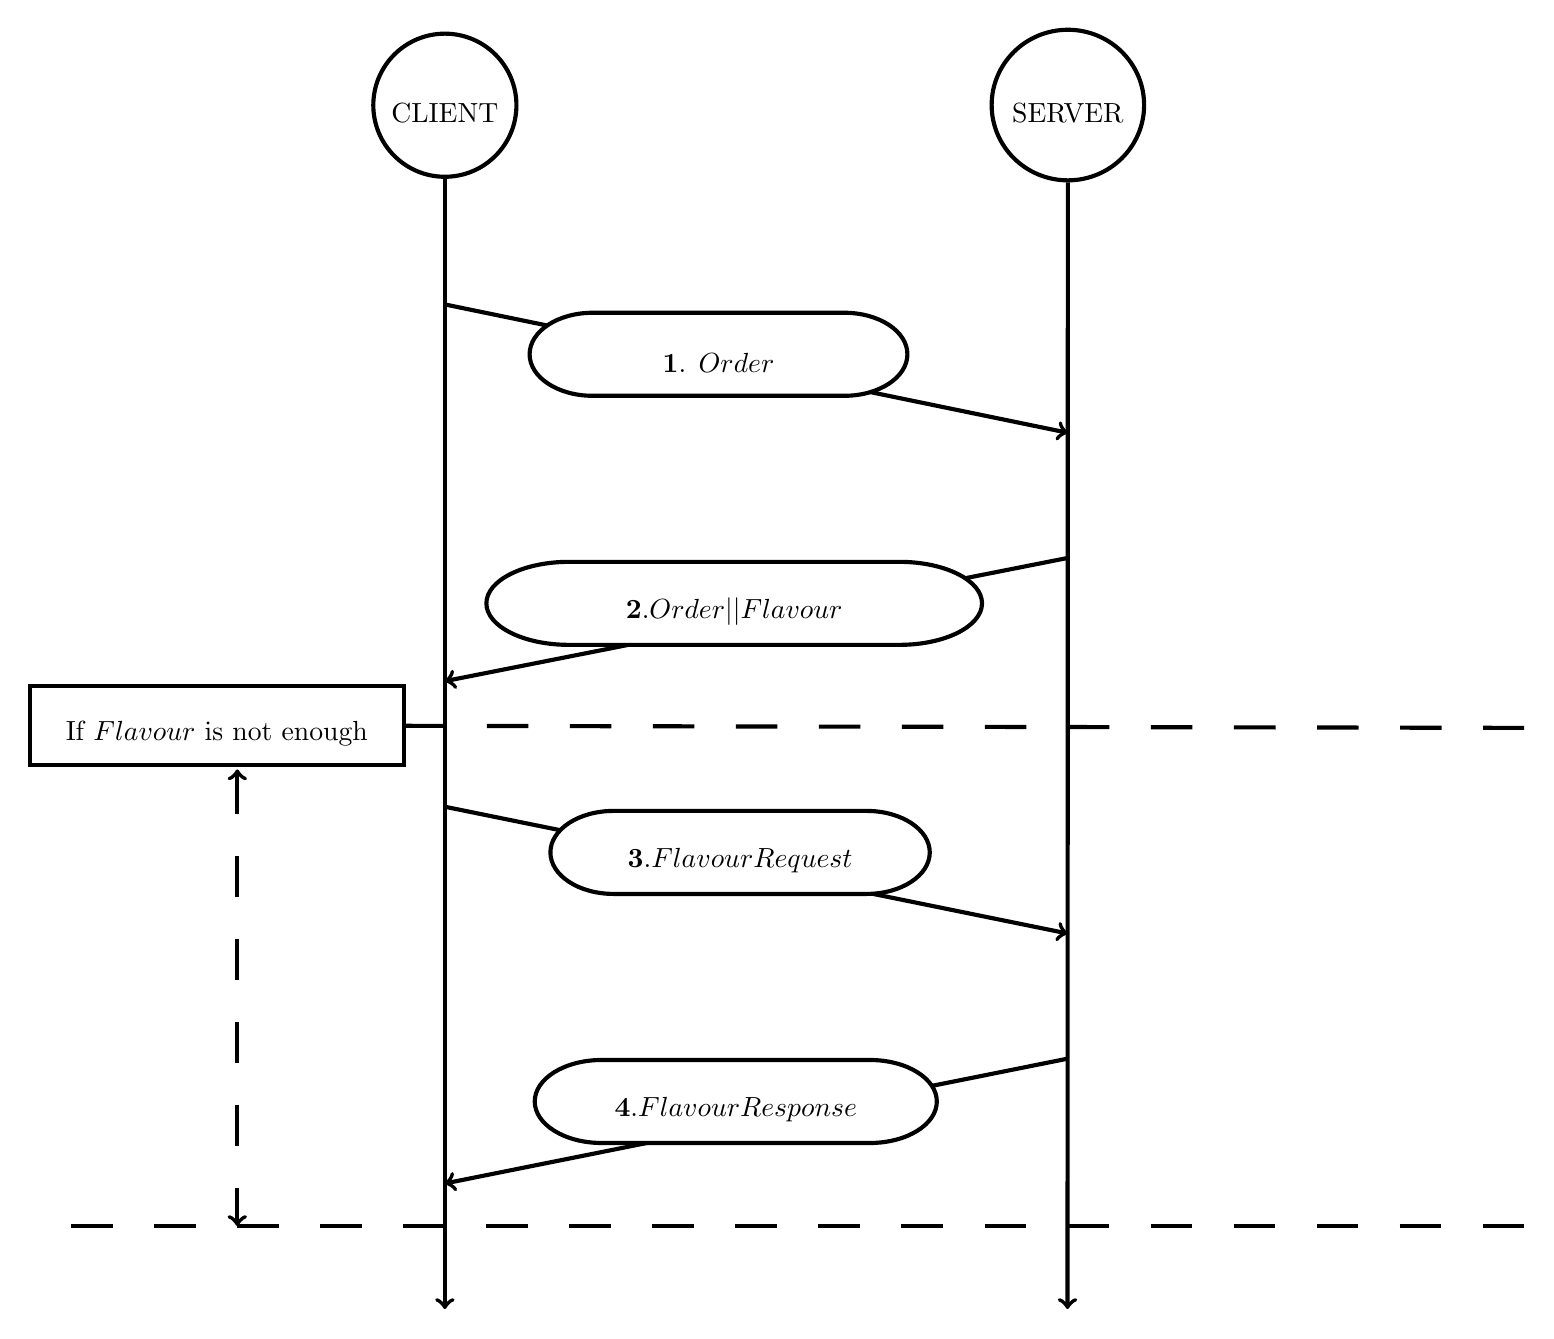
\begin{tikzpicture}
\pgftransformxscale{1.000000}
\pgftransformyscale{-1.000000}
\definecolor{dialinecolor}{rgb}{0.000000, 0.000000, 0.000000}
\pgfsetstrokecolor{dialinecolor}
\definecolor{dialinecolor}{rgb}{1.000000, 1.000000, 1.000000}
\pgfsetfillcolor{dialinecolor}
\definecolor{dialinecolor}{rgb}{1.000000, 1.000000, 1.000000}
\pgfsetfillcolor{dialinecolor}
\pgfpathellipse{\pgfpoint{10.000000\du}{11.000000\du}}{\pgfpoint{1.723870\du}{0\du}}{\pgfpoint{0\du}{1.723870\du}}
\pgfusepath{fill}
\pgfsetlinewidth{0.100000\du}
\pgfsetdash{}{0pt}
\pgfsetdash{}{0pt}
\pgfsetmiterjoin
\definecolor{dialinecolor}{rgb}{0.000000, 0.000000, 0.000000}
\pgfsetstrokecolor{dialinecolor}
\pgfpathellipse{\pgfpoint{10.000000\du}{11.000000\du}}{\pgfpoint{1.723870\du}{0\du}}{\pgfpoint{0\du}{1.723870\du}}
\pgfusepath{stroke}
% setfont left to latex
\definecolor{dialinecolor}{rgb}{0.000000, 0.000000, 0.000000}
\pgfsetstrokecolor{dialinecolor}
\node at (10.000000\du,11.195000\du){CLIENT};
% setfont left to latex
\definecolor{dialinecolor}{rgb}{0.000000, 0.000000, 0.000000}
\pgfsetstrokecolor{dialinecolor}
\node[anchor=west] at (10.000000\du,11.000000\du){};
\definecolor{dialinecolor}{rgb}{1.000000, 1.000000, 1.000000}
\pgfsetfillcolor{dialinecolor}
\pgfpathellipse{\pgfpoint{25.008494\du}{10.996126\du}}{\pgfpoint{1.836494\du}{0\du}}{\pgfpoint{0\du}{1.813886\du}}
\pgfusepath{fill}
\pgfsetlinewidth{0.100000\du}
\pgfsetdash{}{0pt}
\pgfsetdash{}{0pt}
\pgfsetmiterjoin
\definecolor{dialinecolor}{rgb}{0.000000, 0.000000, 0.000000}
\pgfsetstrokecolor{dialinecolor}
\pgfpathellipse{\pgfpoint{25.008494\du}{10.996126\du}}{\pgfpoint{1.836494\du}{0\du}}{\pgfpoint{0\du}{1.813886\du}}
\pgfusepath{stroke}
% setfont left to latex
\definecolor{dialinecolor}{rgb}{0.000000, 0.000000, 0.000000}
\pgfsetstrokecolor{dialinecolor}
\node at (25.008494\du,11.191126\du){SERVER};
\pgfsetlinewidth{0.100000\du}
\pgfsetdash{}{0pt}
\pgfsetdash{}{0pt}
\pgfsetbuttcap
{
\definecolor{dialinecolor}{rgb}{0.000000, 0.000000, 0.000000}
\pgfsetfillcolor{dialinecolor}
% was here!!!
\pgfsetarrowsend{to}
\definecolor{dialinecolor}{rgb}{0.000000, 0.000000, 0.000000}
\pgfsetstrokecolor{dialinecolor}
\draw (10.000000\du,12.774002\du)--(10.000000\du,40.000000\du);
}
\pgfsetlinewidth{0.100000\du}
\pgfsetdash{}{0pt}
\pgfsetdash{}{0pt}
\pgfsetbuttcap
{
\definecolor{dialinecolor}{rgb}{0.000000, 0.000000, 0.000000}
\pgfsetfillcolor{dialinecolor}
% was here!!!
\pgfsetarrowsend{to}
\definecolor{dialinecolor}{rgb}{0.000000, 0.000000, 0.000000}
\pgfsetstrokecolor{dialinecolor}
\draw (25.007949\du,12.859321\du)--(25.000000\du,40.000000\du);
}
\pgfsetlinewidth{0.100000\du}
\pgfsetdash{}{0pt}
\pgfsetdash{}{0pt}
\pgfsetbuttcap
{
\definecolor{dialinecolor}{rgb}{0.000000, 0.000000, 0.000000}
\pgfsetfillcolor{dialinecolor}
% was here!!!
\pgfsetarrowsend{to}
\definecolor{dialinecolor}{rgb}{0.000000, 0.000000, 0.000000}
\pgfsetstrokecolor{dialinecolor}
\draw (10.000000\du,15.799100\du)--(25.006200\du,18.890600\du);
}
\pgfsetlinewidth{0.100000\du}
\pgfsetdash{}{0pt}
\pgfsetdash{}{0pt}
\pgfsetbuttcap
{
\definecolor{dialinecolor}{rgb}{0.000000, 0.000000, 0.000000}
\pgfsetfillcolor{dialinecolor}
% was here!!!
\pgfsetarrowsend{to}
\definecolor{dialinecolor}{rgb}{0.000000, 0.000000, 0.000000}
\pgfsetstrokecolor{dialinecolor}
\draw (25.005300\du,21.906200\du)--(10.000000\du,24.874400\du);
}
\pgfsetlinewidth{0.100000\du}
\pgfsetdash{}{0pt}
\pgfsetdash{}{0pt}
\pgfsetbuttcap
\pgfsetmiterjoin
\pgfsetlinewidth{0.100000\du}
\pgfsetbuttcap
\pgfsetmiterjoin
\pgfsetdash{}{0pt}
\definecolor{dialinecolor}{rgb}{1.000000, 1.000000, 1.000000}
\pgfsetfillcolor{dialinecolor}
\pgfpathmoveto{\pgfpoint{13.558175\du}{16.000000\du}}
\pgfpathlineto{\pgfpoint{19.625675\du}{16.000000\du}}
\pgfpathcurveto{\pgfpoint{20.463422\du}{16.000000\du}}{\pgfpoint{21.142550\du}{16.447715\du}}{\pgfpoint{21.142550\du}{17.000000\du}}
\pgfpathcurveto{\pgfpoint{21.142550\du}{17.552285\du}}{\pgfpoint{20.463422\du}{18.000000\du}}{\pgfpoint{19.625675\du}{18.000000\du}}
\pgfpathlineto{\pgfpoint{13.558175\du}{18.000000\du}}
\pgfpathcurveto{\pgfpoint{12.720428\du}{18.000000\du}}{\pgfpoint{12.041300\du}{17.552285\du}}{\pgfpoint{12.041300\du}{17.000000\du}}
\pgfpathcurveto{\pgfpoint{12.041300\du}{16.447715\du}}{\pgfpoint{12.720428\du}{16.000000\du}}{\pgfpoint{13.558175\du}{16.000000\du}}
\pgfusepath{fill}
\definecolor{dialinecolor}{rgb}{0.000000, 0.000000, 0.000000}
\pgfsetstrokecolor{dialinecolor}
\pgfpathmoveto{\pgfpoint{13.558175\du}{16.000000\du}}
\pgfpathlineto{\pgfpoint{19.625675\du}{16.000000\du}}
\pgfpathcurveto{\pgfpoint{20.463422\du}{16.000000\du}}{\pgfpoint{21.142550\du}{16.447715\du}}{\pgfpoint{21.142550\du}{17.000000\du}}
\pgfpathcurveto{\pgfpoint{21.142550\du}{17.552285\du}}{\pgfpoint{20.463422\du}{18.000000\du}}{\pgfpoint{19.625675\du}{18.000000\du}}
\pgfpathlineto{\pgfpoint{13.558175\du}{18.000000\du}}
\pgfpathcurveto{\pgfpoint{12.720428\du}{18.000000\du}}{\pgfpoint{12.041300\du}{17.552285\du}}{\pgfpoint{12.041300\du}{17.000000\du}}
\pgfpathcurveto{\pgfpoint{12.041300\du}{16.447715\du}}{\pgfpoint{12.720428\du}{16.000000\du}}{\pgfpoint{13.558175\du}{16.000000\du}}
\pgfusepath{stroke}
% setfont left to latex
\definecolor{dialinecolor}{rgb}{0.000000, 0.000000, 0.000000}
\pgfsetstrokecolor{dialinecolor}
\node at (16.591925\du,17.200000\du){\textbf{1}. $Order$};
\pgfsetlinewidth{0.100000\du}
\pgfsetdash{}{0pt}
\pgfsetdash{}{0pt}
\pgfsetbuttcap
\pgfsetmiterjoin
\pgfsetlinewidth{0.100000\du}
\pgfsetbuttcap
\pgfsetmiterjoin
\pgfsetdash{}{0pt}
\definecolor{dialinecolor}{rgb}{1.000000, 1.000000, 1.000000}
\pgfsetfillcolor{dialinecolor}
\pgfpathmoveto{\pgfpoint{12.990000\du}{22.000000\du}}
\pgfpathlineto{\pgfpoint{20.950000\du}{22.000000\du}}
\pgfpathcurveto{\pgfpoint{22.049047\du}{22.000000\du}}{\pgfpoint{22.940000\du}{22.447715\du}}{\pgfpoint{22.940000\du}{23.000000\du}}
\pgfpathcurveto{\pgfpoint{22.940000\du}{23.552285\du}}{\pgfpoint{22.049047\du}{24.000000\du}}{\pgfpoint{20.950000\du}{24.000000\du}}
\pgfpathlineto{\pgfpoint{12.990000\du}{24.000000\du}}
\pgfpathcurveto{\pgfpoint{11.890953\du}{24.000000\du}}{\pgfpoint{11.000000\du}{23.552285\du}}{\pgfpoint{11.000000\du}{23.000000\du}}
\pgfpathcurveto{\pgfpoint{11.000000\du}{22.447715\du}}{\pgfpoint{11.890953\du}{22.000000\du}}{\pgfpoint{12.990000\du}{22.000000\du}}
\pgfusepath{fill}
\definecolor{dialinecolor}{rgb}{0.000000, 0.000000, 0.000000}
\pgfsetstrokecolor{dialinecolor}
\pgfpathmoveto{\pgfpoint{12.990000\du}{22.000000\du}}
\pgfpathlineto{\pgfpoint{20.950000\du}{22.000000\du}}
\pgfpathcurveto{\pgfpoint{22.049047\du}{22.000000\du}}{\pgfpoint{22.940000\du}{22.447715\du}}{\pgfpoint{22.940000\du}{23.000000\du}}
\pgfpathcurveto{\pgfpoint{22.940000\du}{23.552285\du}}{\pgfpoint{22.049047\du}{24.000000\du}}{\pgfpoint{20.950000\du}{24.000000\du}}
\pgfpathlineto{\pgfpoint{12.990000\du}{24.000000\du}}
\pgfpathcurveto{\pgfpoint{11.890953\du}{24.000000\du}}{\pgfpoint{11.000000\du}{23.552285\du}}{\pgfpoint{11.000000\du}{23.000000\du}}
\pgfpathcurveto{\pgfpoint{11.000000\du}{22.447715\du}}{\pgfpoint{11.890953\du}{22.000000\du}}{\pgfpoint{12.990000\du}{22.000000\du}}
\pgfusepath{stroke}
% setfont left to latex
\definecolor{dialinecolor}{rgb}{0.000000, 0.000000, 0.000000}
\pgfsetstrokecolor{dialinecolor}
\node at (16.970000\du,23.200000\du){\textbf{2}.$Order || Flavour$};
\pgfsetlinewidth{0.100000\du}
\pgfsetdash{{1.000000\du}{1.000000\du}}{0\du}
\pgfsetdash{{1.000000\du}{1.000000\du}}{0\du}
\pgfsetbuttcap
{
\definecolor{dialinecolor}{rgb}{0.000000, 0.000000, 0.000000}
\pgfsetfillcolor{dialinecolor}
% was here!!!
\definecolor{dialinecolor}{rgb}{0.000000, 0.000000, 0.000000}
\pgfsetstrokecolor{dialinecolor}
\draw (9.010000\du,25.950000\du)--(36.000000\du,26.000000\du);
}
\definecolor{dialinecolor}{rgb}{1.000000, 1.000000, 1.000000}
\pgfsetfillcolor{dialinecolor}
\fill (0.000000\du,25.000000\du)--(0.000000\du,26.900000\du)--(9.010000\du,26.900000\du)--(9.010000\du,25.000000\du)--cycle;
\pgfsetlinewidth{0.100000\du}
\pgfsetdash{}{0pt}
\pgfsetdash{}{0pt}
\pgfsetmiterjoin
\definecolor{dialinecolor}{rgb}{0.000000, 0.000000, 0.000000}
\pgfsetstrokecolor{dialinecolor}
\draw (0.000000\du,25.000000\du)--(0.000000\du,26.900000\du)--(9.010000\du,26.900000\du)--(9.010000\du,25.000000\du)--cycle;
% setfont left to latex
\definecolor{dialinecolor}{rgb}{0.000000, 0.000000, 0.000000}
\pgfsetstrokecolor{dialinecolor}
\node at (4.505000\du,26.145000\du){If $Flavour$ is not enough};
\pgfsetlinewidth{0.100000\du}
\pgfsetdash{}{0pt}
\pgfsetdash{}{0pt}
\pgfsetbuttcap
{
\definecolor{dialinecolor}{rgb}{0.000000, 0.000000, 0.000000}
\pgfsetfillcolor{dialinecolor}
% was here!!!
\pgfsetarrowsend{to}
\definecolor{dialinecolor}{rgb}{0.000000, 0.000000, 0.000000}
\pgfsetstrokecolor{dialinecolor}
\draw (10.000000\du,27.899600\du)--(25.002700\du,30.953100\du);
}
\pgfsetlinewidth{0.100000\du}
\pgfsetdash{}{0pt}
\pgfsetdash{}{0pt}
\pgfsetbuttcap
\pgfsetmiterjoin
\pgfsetlinewidth{0.100000\du}
\pgfsetbuttcap
\pgfsetmiterjoin
\pgfsetdash{}{0pt}
\definecolor{dialinecolor}{rgb}{1.000000, 1.000000, 1.000000}
\pgfsetfillcolor{dialinecolor}
\pgfpathmoveto{\pgfpoint{14.065625\du}{28.000000\du}}
\pgfpathlineto{\pgfpoint{20.158125\du}{28.000000\du}}
\pgfpathcurveto{\pgfpoint{20.999324\du}{28.000000\du}}{\pgfpoint{21.681250\du}{28.447715\du}}{\pgfpoint{21.681250\du}{29.000000\du}}
\pgfpathcurveto{\pgfpoint{21.681250\du}{29.552285\du}}{\pgfpoint{20.999324\du}{30.000000\du}}{\pgfpoint{20.158125\du}{30.000000\du}}
\pgfpathlineto{\pgfpoint{14.065625\du}{30.000000\du}}
\pgfpathcurveto{\pgfpoint{13.224426\du}{30.000000\du}}{\pgfpoint{12.542500\du}{29.552285\du}}{\pgfpoint{12.542500\du}{29.000000\du}}
\pgfpathcurveto{\pgfpoint{12.542500\du}{28.447715\du}}{\pgfpoint{13.224426\du}{28.000000\du}}{\pgfpoint{14.065625\du}{28.000000\du}}
\pgfusepath{fill}
\definecolor{dialinecolor}{rgb}{0.000000, 0.000000, 0.000000}
\pgfsetstrokecolor{dialinecolor}
\pgfpathmoveto{\pgfpoint{14.065625\du}{28.000000\du}}
\pgfpathlineto{\pgfpoint{20.158125\du}{28.000000\du}}
\pgfpathcurveto{\pgfpoint{20.999324\du}{28.000000\du}}{\pgfpoint{21.681250\du}{28.447715\du}}{\pgfpoint{21.681250\du}{29.000000\du}}
\pgfpathcurveto{\pgfpoint{21.681250\du}{29.552285\du}}{\pgfpoint{20.999324\du}{30.000000\du}}{\pgfpoint{20.158125\du}{30.000000\du}}
\pgfpathlineto{\pgfpoint{14.065625\du}{30.000000\du}}
\pgfpathcurveto{\pgfpoint{13.224426\du}{30.000000\du}}{\pgfpoint{12.542500\du}{29.552285\du}}{\pgfpoint{12.542500\du}{29.000000\du}}
\pgfpathcurveto{\pgfpoint{12.542500\du}{28.447715\du}}{\pgfpoint{13.224426\du}{28.000000\du}}{\pgfpoint{14.065625\du}{28.000000\du}}
\pgfusepath{stroke}
% setfont left to latex
\definecolor{dialinecolor}{rgb}{0.000000, 0.000000, 0.000000}
\pgfsetstrokecolor{dialinecolor}
\node at (17.111875\du,29.200000\du){\textbf{3}.$FlavourRequest$};
\pgfsetlinewidth{0.100000\du}
\pgfsetdash{{1.000000\du}{1.000000\du}}{0\du}
\pgfsetdash{{1.000000\du}{1.000000\du}}{0\du}
\pgfsetbuttcap
{
\definecolor{dialinecolor}{rgb}{0.000000, 0.000000, 0.000000}
\pgfsetfillcolor{dialinecolor}
% was here!!!
\definecolor{dialinecolor}{rgb}{0.000000, 0.000000, 0.000000}
\pgfsetstrokecolor{dialinecolor}
\draw (1.000000\du,38.000000\du)--(36.000000\du,38.000000\du);
}
\pgfsetlinewidth{0.100000\du}
\pgfsetdash{}{0pt}
\pgfsetdash{}{0pt}
\pgfsetbuttcap
{
\definecolor{dialinecolor}{rgb}{0.000000, 0.000000, 0.000000}
\pgfsetfillcolor{dialinecolor}
% was here!!!
\pgfsetarrowsend{to}
\definecolor{dialinecolor}{rgb}{0.000000, 0.000000, 0.000000}
\pgfsetstrokecolor{dialinecolor}
\draw (25.001800\du,33.968700\du)--(10.000000\du,36.974900\du);
}
\pgfsetlinewidth{0.100000\du}
\pgfsetdash{}{0pt}
\pgfsetdash{}{0pt}
\pgfsetbuttcap
\pgfsetmiterjoin
\pgfsetlinewidth{0.100000\du}
\pgfsetbuttcap
\pgfsetmiterjoin
\pgfsetdash{}{0pt}
\definecolor{dialinecolor}{rgb}{1.000000, 1.000000, 1.000000}
\pgfsetfillcolor{dialinecolor}
\pgfpathmoveto{\pgfpoint{13.779375\du}{34.000000\du}}
\pgfpathlineto{\pgfpoint{20.236875\du}{34.000000\du}}
\pgfpathcurveto{\pgfpoint{21.128470\du}{34.000000\du}}{\pgfpoint{21.851250\du}{34.447715\du}}{\pgfpoint{21.851250\du}{35.000000\du}}
\pgfpathcurveto{\pgfpoint{21.851250\du}{35.552285\du}}{\pgfpoint{21.128470\du}{36.000000\du}}{\pgfpoint{20.236875\du}{36.000000\du}}
\pgfpathlineto{\pgfpoint{13.779375\du}{36.000000\du}}
\pgfpathcurveto{\pgfpoint{12.887780\du}{36.000000\du}}{\pgfpoint{12.165000\du}{35.552285\du}}{\pgfpoint{12.165000\du}{35.000000\du}}
\pgfpathcurveto{\pgfpoint{12.165000\du}{34.447715\du}}{\pgfpoint{12.887780\du}{34.000000\du}}{\pgfpoint{13.779375\du}{34.000000\du}}
\pgfusepath{fill}
\definecolor{dialinecolor}{rgb}{0.000000, 0.000000, 0.000000}
\pgfsetstrokecolor{dialinecolor}
\pgfpathmoveto{\pgfpoint{13.779375\du}{34.000000\du}}
\pgfpathlineto{\pgfpoint{20.236875\du}{34.000000\du}}
\pgfpathcurveto{\pgfpoint{21.128470\du}{34.000000\du}}{\pgfpoint{21.851250\du}{34.447715\du}}{\pgfpoint{21.851250\du}{35.000000\du}}
\pgfpathcurveto{\pgfpoint{21.851250\du}{35.552285\du}}{\pgfpoint{21.128470\du}{36.000000\du}}{\pgfpoint{20.236875\du}{36.000000\du}}
\pgfpathlineto{\pgfpoint{13.779375\du}{36.000000\du}}
\pgfpathcurveto{\pgfpoint{12.887780\du}{36.000000\du}}{\pgfpoint{12.165000\du}{35.552285\du}}{\pgfpoint{12.165000\du}{35.000000\du}}
\pgfpathcurveto{\pgfpoint{12.165000\du}{34.447715\du}}{\pgfpoint{12.887780\du}{34.000000\du}}{\pgfpoint{13.779375\du}{34.000000\du}}
\pgfusepath{stroke}
% setfont left to latex
\definecolor{dialinecolor}{rgb}{0.000000, 0.000000, 0.000000}
\pgfsetstrokecolor{dialinecolor}
\node at (17.008125\du,35.200000\du){\textbf{4}.$FlavourResponse$};
\pgfsetlinewidth{0.100000\du}
\pgfsetdash{{1.000000\du}{1.000000\du}}{0\du}
\pgfsetdash{{1.000000\du}{1.000000\du}}{0\du}
\pgfsetbuttcap
{
\definecolor{dialinecolor}{rgb}{0.000000, 0.000000, 0.000000}
\pgfsetfillcolor{dialinecolor}
% was here!!!
\pgfsetarrowsstart{to}
\pgfsetarrowsend{to}
\definecolor{dialinecolor}{rgb}{0.000000, 0.000000, 0.000000}
\pgfsetstrokecolor{dialinecolor}
\draw (5.000000\du,27.000000\du)--(5.000000\du,38.000000\du);
}
\end{tikzpicture}
